%
% Software.tex
%
% LulzBot Mini User Manual
%
% Copyright (C) 2014 Aleph Objects, Inc.
%
% This document is licensed under the Creative Commons Attribution 4.0
% International Public License (CC BY-SA 4.0) by Aleph Objects, Inc.
%

\section{Software Overview}
\index{software}

Aleph Objects, Inc., the maker of the LulzBot\textsuperscript{\miniscule{\texttrademark}} Mini, completely supports free/libre hardware and software. Along with the Mini being a free/libre hardware design, it has been tested to work with 100\% free/libre software. Our source code and design files are hosted on our development server found at \texttt{http://devel.lulzbot.com}.
\glossary{free/libre}{Free/Libre hardware and software can be thought of as "free as in free speech, not just free as in free beer", although most free/libre software is available for no cost. Libre hardware designs can be copied, modified and are usually available for download. Free/Libre software can be used in a similar fashion.}
To operate your desktop 3D printer you will need to install a few software packages onto your PC. You will need a 3D printer host, an \texttt{.STL} to \texttt{.gcode} generator, and optional CAD or 3D modeling software.
\glossary{.gcode}{The file extension for G-Code files}
\glossary{GCODE}{The common name for the most widely used CNC programming language.}
\glossary{CAD}{Computer Aided Design}

\index{GNU/Linux}
\index{Apple OS X}
\index{Windows}
\index{operating system}
All of the following free/libre software packages are available for GNU/Linux, Windows, and Apple OS X. However, we highly recommend using these programs on GNU/Linux.

\index{download}
The required software can be found in the Support/Downloads section at \texttt{LulzBot.com/support/downloads}. You will also find instructions there for installing each program onto your PC. You can also find downloads specific to the LulzBot\textsuperscript{\miniscule{\texttrademark}} Mini 3D printer on the LulzBot\textsuperscript{\miniscule{\texttrademark}} Mini product page.

\index{driver}
\section{Installing Drivers}
Linux and Mac OSX users will not need to install a driver to communicate with the Mini 3D printer. Windows users will need to install the following drivers. The drivers can be downloaded from \texttt{LulzBot.com/support/downloads}. A visual guide showing the driver installation process can be found in our download section as well.

\index{pronterface}
\index{printrun}
\index{pronsole}
\index{plater}
\index{stl}
\index{extruder}
\index{extrusion}
\index{temperature}
\index{gcode}
\index{SD card}
\section{Printrun}
\label{Printrun}
Website: \texttt{http://www.github.com/kliment/Printrun}

The host software, Printrun, can be used to start up and control your 3D printer 
(Figure \ref{fig:printrun}, page \pageref{fig:printrun}).
\begin{figure}[hbt]
\centering
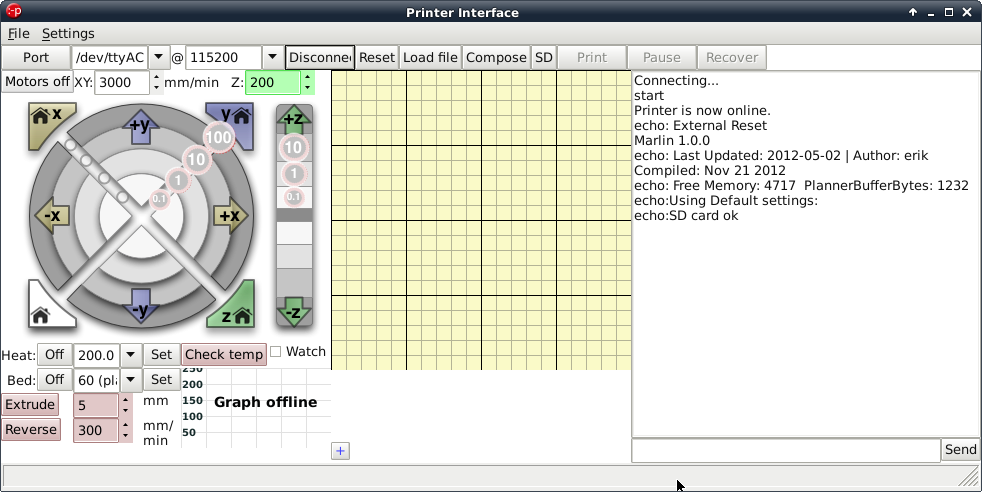
\includegraphics[keepaspectratio=true,angle=0,height=0.4\textheight,width=1.0\textwidth]{printrun.png}
\caption{Printrun application for 3D printer control}
\label{fig:printrun}
\end{figure}
The host controls include: setting the extruder and print surface temperatures, manual control of each axis, and manual extrusion. The host is also where you can push print files (\texttt{.gcode}) to the 3D printer or load print files from the SD card for printing out model designs.

\subsection{Installing Printrun}
Printrun contains several different applications that can be used to control the TAZ 3D printer. It can be installed on Windows, Mac OSX and Linux based computers. We recommend using Pronterface, the graphical user interface for printrun, when setting up or troubleshooting the 3D printer. \texttt{Pronsole} allows printing from the command line, and can be used for scripting and some automation. \texttt{Plater} allows you to arrange and combine several STL files into one. More information on the other programs within the Printrun package can be found at \texttt{https://github.com/kliment/Printrun}. Printrun can be downloaded from \texttt{LulzBot.com/support/downloads}. Download the version for your operating system and extract. You will need an archive manager to extract the files. If you do not have one installed we recommend using 7-zip, which can be downloaded for free at \texttt{www.7-zip.org}.

\begin{itemize}
\subsection{Windows Instructions}
\index{windows}
\item Once downloaded, extract the \texttt{dist} folder to a location of your choice. You can rename the \texttt{dist} folder if you like. Double click \texttt{pronterface.exe} to run Pronterface.


\subsection{Mac OSX Instructions}
\item Once downloaded, extract the \texttt{dist} folder to a location of your choice. Once extracted, double click the \texttt{pronterface-mac-Mar2012.app} file to install.

\subsection{Linux Instructions}
%\begin{itemize}
\subsubsection{Debian|Ubuntu}
\subsubsection{Recommended Installation}
\item We recommend using the stand-alone Printrun option found at \texttt{https://www.LulzBot.com/?=support/downloads}. Once downloaded and extracted, navigate to the extracted directory. Install the dependencies by issuing the following command in a terminal: \texttt{sudo apt-get install python-serial python-wxgtk2.8 python-pyglet}. Once the dependencies have been installed, run Pronterface by using the following command in a terminal: \texttt{python pronterface.py}.

\subsubsection{Installing from source}
\item Using Git, in a terminal issue the following command: \texttt{git clone https://github.com/kliment/Printrun.git}
\item Once downloaded, change to the Printrun directory. You will need to ensure that the following dependencies are met. They are listed in the README.md file. You can use this command to install the dependencies: 
\texttt{sudo apt-get install python-serial python-wxgtk2.8 python-pyglet python-tornado python-setuptools python-libxml2 python-gobject python-pip avahi-daemon libavahi-compat-libdnssd1}
followed by:
\texttt{pip install -r requirements.txt}
To install in a terminal issue the following command:
\texttt{sudo python setup.py install}.
Run Printrun by issuing the following command:
\texttt{python pronterface.py}

\subsubsection{Fedora}
\item Use this command to install Printrun from the official sources: \texttt{sudo yum install printrun}

\subsubsection{Archlinux}
\item Use this command to install Printun from AUR: \texttt{yaourt printrun}

\end{itemize}

\index{printrun}
\section{Using Printrun}

%\begin{figure}[hbt]
\begin{figure}[H]
\centering
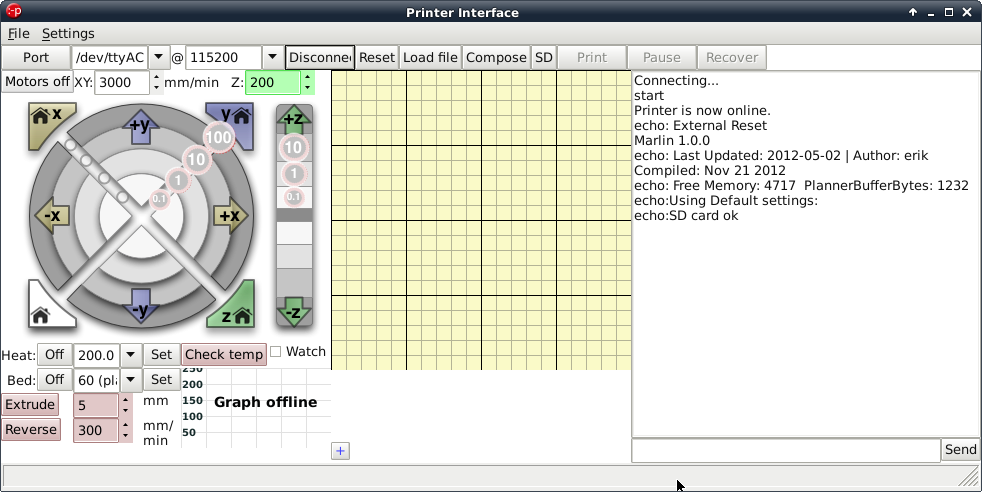
\includegraphics[keepaspectratio=true,angle=0,height=0.4\textheight,width=1.0\textwidth]{printrun.png}
\caption{Printrun}
\label{fig:printrun}
\end{figure}

Printrun is used to control the printer from a computer. It is divided into 4 main parts: The buttons over the top are used to connect to the printer, load files and start \& stop prints.

The movement controls are on the left hand side, with the G-code preview window in the center and the Log window and Terminal command entry box on the right hand side (Figure \ref{fig:printrun}, page \pageref{fig:printrun}).

\subsection{Connecting to the TAZ 3D Printer}
\index{connecting}
\index{Printrun}
\index{USB cable}
\index{port}
\index{baud rate}
\glossary{Baud Rate}{Refers to the speed at which the host controller communicates with the 3d Printer electronics.}
To start up the printer, first you will need to connect to the printer with Printrun. Make sure you have connected the USB cable from your PC to the printer before launching Printrun. If not, close Printrun, connect the USB cable, and relaunch Printrun. To connect to the printer, select the correct port by using the drop down arrow and selecting the active port, generally \texttt{/dev/ttyACM0}). On other operating systems the port may be named such as \texttt{COM1} or \texttt{tty.usbserial-USB-ID}. The \texttt{Port} button will refresh the Port listing. Once selected choose the default \texttt{115200} buad rate and press \texttt{Connect}. Pronterface will open a connection to the printer and display firmware information in the Log window. 

In the text output window you will see multiple return lines. If you see \texttt{Printer is now online} you have successfully connected to the printer. The printer control buttons on the left will also darken and become click-able after connecting. If nothing is displayed in the Log window verify you have the correct port and connection speed selected. When you need to disconnect the printer simply press the \texttt{Disconnect} button.

%\begin{figure}[hbt]
\begin{figure}[H]
\centering
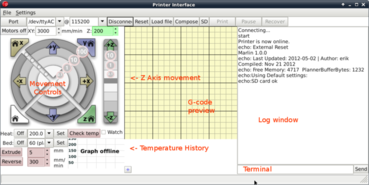
\includegraphics[keepaspectratio=true,angle=0,height=0.4\textheight,width=1.0\textwidth]{printrun-labels.png}
\caption{Printrun Functions}
\label{fig:printrun-labels}
\end{figure}

\subsection{Movement} 
%\begin{figure}[hbt]
\begin{figure}[H]
\centering
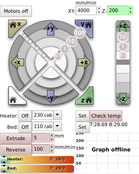
\includegraphics[keepaspectratio=true,angle=0,height=0.4\textheight,width=1.0\textwidth]{printrun_controls.png}
\caption{Movement Controls}
\label{fig:printrun_controls}
\end{figure}

\subsubsection{Motors off}
The TAZ 3D printer can be moved on all three axes independently. If you would like to do so by hand, use the \texttt{Motors off} button to unlock all the stepper motors. Once unlocked they can be moved by hand. Keep in mind that there is no positional feedback, so if you move an axis you will need to re-home in order to re-establish the hot end's position. 

\subsubsection{mm/min XY:/ Z:}
These settings control the manual jog speeds when driven with Pronterface. Use caution when changing these figures. Moving the axes too fast can cause the printer to miss steps. If that occurs with the Z axis, it can potentially cause the Z axis to become out of square.

\subsubsection{Homing}
\index{end stops}
Caution: when homing, the axis will continue to move in the negative direction until the end stop switch is activated. If the printer is ever transported make sure the end stop switches are clear before resuming printing. If an axis has missed an end stop and is continuing to try to move in the negative direction, immediately turn the power switch to the off position. 

Each axes can be homed either individually or together. Press the \texttt{Home X} button to move the X axis to the left until it activates the end stop. Once the X axis end stop is activated, the X axis carriage will 'bounce'- it will move over and move back to the home position more slowly. Press the \texttt{Home Y} button to home the Y axis. The Y axis platform will move away from you towards the rear of the printer. The Z home button functions the same, but the Z trigger can be adjusted manually on the printer. \textcolor{red}{DO NOT press the \texttt{Home Z} button to home the Z axis or the \texttt{Home All button} at this time.} In a later step you will need to set the Z end stop trigger before homing Z.

\subsubsection{X/Y/Z Axes Movement Controls}
Prior to moving the X, Y, or Z axis, make sure that you home each axis. The X, Y and Z axes can be moved utilizing the circular movement controls. Each axis can be moved in either fine moves or large moves, ranging from 0.1mm to 100mm.  For example, to move the \texttt{Y Axis} towards you, move your mouse to the \texttt{+y} section until both the \texttt{+y} and the \texttt{100} are highlighted then select that ring section. To move the \texttt{Y axis} away from you, move your mouse to the \texttt{-y} section until both the \texttt{-y} and the \texttt{100} are highlighted then select that ring section. The X axis can be moved in a similar fashion.

\textcolor{red}{DO NOT press the \texttt{Home Z} button to home the Z axis or the \texttt{Home All button} at this time.} The Z axis movement control operates similarly, but the movement scale is different. The Z axis will move in 0.1mm, 1mm and 10mm increments. The top half of the movement bar will move the Z axis up, by the selected units, while the lower half will move the Z axis down, by the selected units. 




\begin{comment}
\section{Slic3r}
\index{gcode}
\index{STL}
\glossary{STL}{stereolithography file, also known as standard tessellation language; STL file is the common 3D model file format.}
\index{CAD}
\index{resolution}
\index{Slic3r}
Website:  \texttt{http://www.slic3r.org}

The Slic3r software is the first tool in the chain of 3D printing software
(Figure \ref{fig:slic3r}, page \pageref{fig:slic3r}).
\begin{figure}[hbt]
\centering
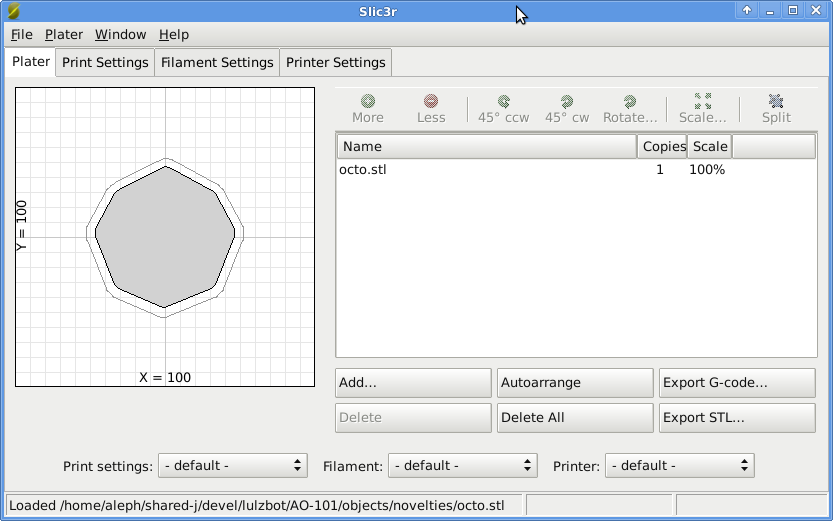
\includegraphics[keepaspectratio=true,angle=0,height=0.4\textheight,width=1.0\textwidth]{slic3r.png}
\caption{Slic3r application, STL to .gcode generator}
\label{fig:slic3r}
\end{figure}

Slic3r uses commonly used \texttt{.STL} files to create \texttt{.gcode} files. Gcode files contain instructions for the 3D printer on where, when, and how quickly to make movements. However, .gcode programming is not very suitable for CAD and 3D design. This is where Slic3r and the \texttt{.STL} file comes into use. The \texttt{.STL} file is a 3D model file that can be exported by all common CAD and 3D modeling software. The Slic3r software then slices the \texttt{.STL} 3D model into layers and print paths to create a 3D-printable \texttt{.gcode} file.

To launch Slic3r navigate to the \texttt{Slic3r} directory and launch the \texttt{slic3r.pl} file. On GNU/Linux operating systems you may need to set the \texttt{slic3r.pl} file as executable. It may be called \texttt{slic3r.exe} on other operating systems.

\index{download}
Slic3r includes very simple settings that allow you to easily refine prints. You can create multiple configurations for changing printer setups including nozzle sizes and desired print resolution. For ease of use we have pre-defined Slic3r configurations. They are available in the Support/Downloads section at \texttt{www.LulzBot.com}. Download the configurations to your \texttt{Slic3r} directory.

\index{configuration}
\subsection{Loading Configurations}
To load configurations, press the \texttt{Load Config...} button. In the file browser that opens, locate the downloaded configuration files. Select the configuration file that matches the nozzle size currently installed on the printer (0.5-mm nozzle is installed by default). Press \texttt{Open} and the pre-defined configuration will load into Slic3r. You can also save custom configurations for yourself by pressing the \texttt{Export Config...} button. A file browser will open that allows you to define a name and save your custom configuration. 

\index{STL}
\index{plater}
\subsection{Loading .STL files}
To load an \texttt{.STL} 3D model file into Slic3r, activate the Plater tab and click the \texttt{Add...} button. In the file browser navigate to the \texttt{.STL} you wish to load and click \texttt{Open}. The silhouette of the model will appear in the Plater diagram. To print more than one copy of the model at a time, select the model name from the list and click the \texttt{More} button. With each press of the \texttt{More} button, an additional copy of the model will be added to Plater. To remove a copy of the model, select the model name again and click \texttt{Less}. To completely remove the model from Plater, select the model name and click \texttt{Delete}.

\index{gcode}
\subsection{Export .gcode files}
Once you have finished setting your part(s) in Plater you can generate the .gcode by clicking \texttt{Export G-Code...}. In the file browser, navigate to where you would like to save the \texttt{.gcode} file and list a name to save the file as. Click \texttt{Save} and Slic3r will begin generating the \texttt{.gcode} file. When Slicer is finished you will receive a prompt. If you have created a plate with multiple model designs, you can also use the \texttt{Export STL...} function to save an \texttt{.STL} file to quickly reproduce the same plate of models.


\section{Printrun}
%%% XXX shouldn't have to do it this way.
%%% HOWTO get page number from section? Ala  sec:Printrun
\label{Printrun}
\index{extruder}
\index{extrusion}
\index{temperature}
\index{gcode}
\index{SD card}
\index{Printrun}
Website: \texttt{http://www.github.com/kliment/Printrun}

The host software, Printrun, can be used to start up and control your 3D printer 
(Figure \ref{fig:printrun}, page \pageref{fig:printrun}).
\begin{figure}[hbt]
\centering
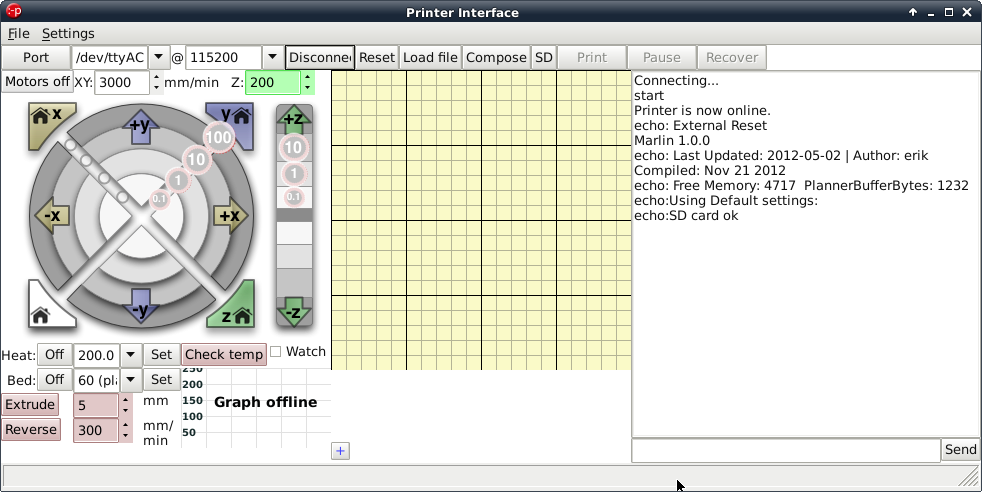
\includegraphics[keepaspectratio=true,angle=0,height=0.4\textheight,width=1.0\textwidth]{printrun.png}
\caption{Printrun application for 3D printer control}
\label{fig:printrun}
\end{figure}
The host controls include: setting the extruder and print surface temperatures, manual control of each axis, and manual extrusion. The host is also where you will push print files (\texttt{.gcode}) to the 3D printer or load print files from the SD card for printing model designs.

\index{pronterface}
\index{GNU/Linux}
To launch Printrun, navigate to the \texttt{Printrun} directory and launch the \texttt{pronterface.py} file. On GNU/Linux operating systems you may need to set the \texttt{pronterface.py} file as executable. Depending on your environment you may need to launch the program by using the full command: \texttt{python pronterface.py}. On other operating systems the file may be called \texttt{pronterface.exe}.

\subsection{Connecting the Printer}
\index{connecting}
\index{Printrun}
\index{USB cable}
\index{port}
\index{baud rate}
\glossary{Baud Rate}{Refers to the speed at which the host controller communicates with the 3d Printer electronics.}
To start up the printer, first you will need to connect to the printer with Printrun. Before launching Printrun, make sure you have connected the USB cable from your PC to the printer. If not, close Printrun, connect the USB cable, and relaunch Printrun. In the top left \texttt{Port}, pull-down menu select the correct port for the printer (generally \texttt{/dev/ttyACM0}). On other operating systems the port may be named \texttt{COM1} or \texttt{tty.usbserial-USB-ID}. If you have only one printer connected, there will only be one port available to select. Make sure the port baud rate is set to \texttt{115200} in the pull-down menu to the right of the port selection. You can refresh the USB ports, by clicking the \texttt{Port} button.

Now, to connect to the printer, click the \texttt{Connect} button. In the text output window you will see multiple return lines. If you see \texttt{Printer is now online} you have successfully connected to the printer. The printer control buttons on the left will also darken and become click-able after connecting. When you need to disconnect the printer simply press the \texttt{Disconnect} button.

\subsection{Printer Controls}
\index{Printrun}
\index{hot end}
All of the printer controls can be found on the left side of the Printrun interface
(Figure  \ref{fig:printrun_controls}, page \pageref{fig:printrun_controls}).
\begin{figure}[hbt]
\centering
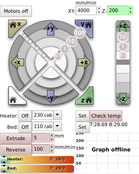
\includegraphics[keepaspectratio=true,angle=0,height=0.4\textheight,width=1.0\textwidth]{printrun_controls.png}
\caption{Printrun controls}
\label{fig:printrun_controls}
\end{figure}
To set the hot end and print surface temperature, first click the \texttt{Monitor Printer} check box on. This will enable the printer temperature bars and graph. The hot end and print surface controls are labeled \texttt{Heater} and \texttt{Bed}. Select the temperature setting by using the pull-down menu for pre-defined temperature settings. You can also set custom temperature settings by typing into the temperature box.

\index{temperature}
To turn on the hot end and/or printer surface, click the respective \texttt{Set} button. The \texttt{Set} button will highlight orange when the temperature is set to "On" for that component. When the hot end or print surface is set to "On" you will see the temperature bar and graph display the set temperature and the current temperature. When both components have reached the correct temperature, the printer is ready for printing. Clicking the \texttt{Off} button will turn off that component and highlight the \texttt{Off} button blue.

\index{extrude}
\index{hot end}
Below the temperature controls are the manual extrusion controls. There you can manually extrude plastic through the hot end and retract the plastic filament from the hot end. The \texttt{Extrude} button will feed the amount of plastic, set to the right in millimeters, into the hot end. The rate at which the plastic is fed is set below the extrusion length (mm/min). The \texttt{Reverse} button will perform the opposite of \texttt{Extrude}, pulling the plastic filament back out of the hot end.

\index{manual controls}
\index{axes}
\index{X axis}
\index{Y axis}
\index{Z axis}
The large pattern of buttons above the temperature controls are the axes manual controls. These functions allow you to manually move each of the three axes of the printer. The circular pattern of four quadrants controls the X and Y axes. The top and bottom quadrants move the Y axis; the top in the positive direction (forward) and the bottom in the negative direction (backward). The left and right quadrants move the X axis; the left in the negative direction (left) and the right in the positive direction (right).

Each quadrant is split into four sections that control the length of movement by 0.1mm, 1mm, 10mm, or 100mm. The innermost section moves the axis 0.1-mm, with each section outwards becoming a larger movement, with the outside section moving the axis 100-mm.

The linear control bar to the right controls the Z axis. The Z axis is also separated into multiple movement lengths: 0.1mm, 1mm, and 10mm. The upper three buttons move the Z axis up and away from the printer surface; the three lower buttons move the Z axis closer to the print surface.

\index{home}
The four triangular buttons around the circular pattern are the axes home buttons. Each home button will move that axis in the negative direction until the end stop is activated. There is a home button for the X, Y, and Z axes. There is also a white "Home ALL" button that homes all of the axes at once.
\end{comment}


\begin{comment}
\subsection{Loading print files}
\index{load files}
\index{gcode}
\index{Printrun}

To load a \texttt{.gcode} file into Printrun click the \texttt{Load file} button. Navigate to the \texttt{.gcode} file in the file browser and click \texttt{Open}. You will now see a 2D image of the first layer of your model design in the .gcode viewer
(Figure \ref{fig:printrun_viewer}, page \pageref{fig:printrun_viewer}).
\begin{figure}[hbt]
\centering
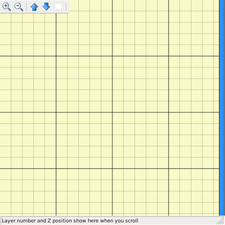
\includegraphics[keepaspectratio=true,angle=0,height=0.4\textheight,width=1.0\textwidth]{printrun_viewer.png}
\caption{Printrun viewer}
\label{fig:printrun_viewer}
\end{figure}
Click the .gcode viewer window to see a more detailed version of the sliced model. In the pop-up .gcode viewer you can zoom in using the mouse scroll wheel and flip through layers with the up and down arrow keys. To pan within the window, left-click and drag to move around the work plane. The lines shown in the .gcode viewer represent the path the extrusion nozzle will follow to print the model.

For more information on using Printrun, see the Printrun page in the Support/Downloads section at \texttt{https://www.lulzbot.com/?q=support}. Instructions for running a print can be found in the Starting the First Print section in this manual.
\end{comment}

\section{CAD and 3D Modeling Software}
\index{CAD}
\index{software}
\index{STL}

LulzBot is not distributing a CAD or 3D modeling software package. However, multiple free/libre software packages are available. Other common non-free CAD and 3D modeling software are also capable of exporting the required \texttt{.STL} files.

On some CAD and 3D modeling software you will need to select millimeters as the output unit. If possible it is best to build your 3D design in metric units rather than imperial units. Slic3r requires .STL files sized in millimeters. If an .STL with inches as units is loaded into the Slic3r, the model will be scaled much smaller than expected. You can scale the model by 2540\% to compensate. The software listed below outputs millimeters as the unit by default.

\subsection{FreeCAD}
\index{FreeCAD}
\index{GNU/Linux}
\index{Windows}
\index{Apple OS X}
Website: \texttt{http://free-cad.sourceforge.net}

Although still in development, FreeCAD is a great free/libre CAD application. Containing a full GUI for building CAD models, FreeCAD is capable of creating simple to complex designs. STL files can also easily be exported for use with 3D printing. FreeCAD is available for GNU/Linux, Windows, and Mac. The latest development version is recommended.

\subsection{OpenSCAD}
\index{OpenSCAD}
\index{GNU/Linux}
\index{Windows}
\index{Apple OS X}
Website: \texttt{http://openscad.org}

OpenSCAD is another free/libre CAD software; however, different than FreeCAD, it is script based. Rather than using a GUI to generate CAD designs, OpenSCAD CAD designs are created using script based renderings. Users with programming experience would find this very useful. Also, OpenSCAD uses a simple script language that is easy for users with little or no programming experience to learn.

\subsection{Blender}
\index{Blender}
\index{GNU/Linux}
\index{Windows}
\index{Apple OS X}
Website: \texttt{http://blender.org}

The most widely used free/libre 3D modeling software, Blender is well documented with tutorials available on the Blender.org website as well as found online.

\subsection{Shapesmith}
\index{Shapesmith}
Website: \texttt{http://shapesmith.net}

Shapesmith is a web-based 3D modeling software. This means there is no required software to get started designing models. Shapesmith is also a great choice for anyone starting out in CAD/ 3D modeling.

\section{Alternative Printer Host Software}
\index{Host}
\index{software}
\index{STL}

\subsection{OctoPrint}
\index{OctoPrint}
\index{GNU/Linux}
\index{Windows}
\index{Apple OS X}
Website: \texttt{http://octoprint.org/}

Octoprint is a printer host that uses a web-based interface to access and control the 3D printer. Added web-cam functionality allows for time-lapse videos and a live stream. Octoprint will run on Windows, Apple and Linux based computers and can even run well on a Beagle Bone Black or a RaspberryPi (inexpensive business-card sized computers). 

\subsection{BotQueue}
\index{BotQueue
\index{GNU/Linux}
\index{Apple OS X}
Website: \texttt{https://www.botqueue.com/}

Botqueue works well for those users wanting to have a web-based multiple 3D printer operation running off a queuing system.


\subsection{MatterControl}
\index{MatterControl}
%\index{GNU/Linux}
\index{Windows}
\index{Apple OS X}
Website: \texttt{http://www.mattercontrol.com/}

MatterControl is another printer host that currently runs on Windows and Apple computers. It features 2D and 3D model viewing, a print queue and print file organization and searching.

